% !TEX program = xelatex
\documentclass[9pt, aspectratio=169]{ctexbeamer}
\usepackage{amsmath,amssymb,booktabs,multirow,colortbl,xcolor,hyperref,tikz,pgfplots}

\definecolor{theme}{RGB}{41,65,130}
\definecolor{titlebg}{RGB}{30,50,100}

\usetheme{Frankfurt}\usecolortheme{beaver}
\setbeamercolor{structure}{fg=theme}
\setbeamercolor{title}{fg=white,bg=titlebg}
\setbeamercolor{frametitle}{fg=theme,bg=gray!10}
\setbeamercolor{block title}{fg=white,bg=theme}
\setbeamercolor{block body}{bg=gray!5}
\setbeamercolor{background canvas}{bg=white}
\setbeamertemplate{navigation symbols}{}
\setbeamersize{text margin left=0.5cm, text margin right=0.5cm}

\title{SGL 自监督图推荐系统\\与 DMLC 改进}
\subtitle{Self-supervised Graph Learning --- SGL Baseline \& DMLC Enhancement}
\author{训练进展汇报}
\date{2026年6月4日}

\begin{document}
\frame{\titlepage}

%% ==================== LightGCN ====================
\section{LightGCN 骨干网络}
\begin{frame}{LightGCN --- 图构建与归一化}
  \textbf{符号:}
  \begin{columns}[t]
    \begin{column}{0.5\textwidth}\footnotesize
      \begin{itemize}
        \item $N$: 用户数, $M$: 物品数
        \item $d$: 嵌入维度, $L$: GCN 层数
        \item $\mathbf{U}^{(0)}\in\mathbb{R}^{N\times d}$: 用户初始嵌入
        \item $\mathbf{I}^{(0)}\in\mathbb{R}^{M\times d}$: 物品初始嵌入
      \end{itemize}
    \end{column}
    \begin{column}{0.5\textwidth}\footnotesize
      \begin{itemize}
        \item $\mathbf{A}$: 邻接矩阵, $\mathbf{D}$: 度矩阵
        \item $\tilde{\mathbf{A}}$: 对称归一化邻接矩阵
        \item $\mathbf{E}^{(l)}$: 第 $l$ 层节点嵌入
        \item $\mathcal{N}(u)$: 用户 $u$ 的邻居物品集
      \end{itemize}
    \end{column}
  \end{columns}

  \vspace{0.3em}
  \textbf{1. 邻接矩阵 (用户-物品二部图):}
  \begin{equation*}
    \mathbf{A} = \begin{pmatrix}\mathbf{0} & \mathbf{R} \\ \mathbf{R}^\top & \mathbf{0}\end{pmatrix},\qquad
    \mathbf{R}_{ui}=1 \text{ 若交互过}
  \end{equation*}

  \textbf{2. 对称归一化:}
  \begin{equation*}
    \tilde{\mathbf{A}} = \mathbf{D}^{-\frac12}\mathbf{A}\mathbf{D}^{-\frac12},\qquad
    \tilde{\mathbf{A}}_{ui} = \frac{1}{\sqrt{|\mathcal{N}(u)|\cdot|\mathcal{N}(i)|}}
  \end{equation*}
\end{frame}

\begin{frame}{LightGCN --- 传播与输出}
  \textbf{3. LightGCN 传播 (去非线性):}
  \begin{align*}
    \mathbf{E}^{(0)} &= [\mathbf{U}^{(0)}; \mathbf{I}^{(0)}] &&\text{初始嵌入拼接} \\
    \mathbf{E}^{(l+1)} &= \tilde{\mathbf{A}}\,\mathbf{E}^{(l)} &&\text{聚合邻居信息},\; l=0,\dots,L-1
  \end{align*}

  \textbf{节点级展开:}
  \begin{equation*}
    \mathbf{e}_u^{(l+1)} = \sum_{i\in\mathcal{N}(u)}\frac{\mathbf{e}_i^{(l)}}{\sqrt{|\mathcal{N}(u)||\mathcal{N}(i)|}},\qquad
    \mathbf{e}_i^{(l+1)} = \sum_{u\in\mathcal{N}(i)}\frac{\mathbf{e}_u^{(l)}}{\sqrt{|\mathcal{N}(i)||\mathcal{N}(u)|}}
  \end{equation*}
  用户 $u$ 聚合相连物品嵌入；物品 $i$ 聚合相连用户嵌入

  \vspace{0.3em}
  \textbf{4. 各层平均 (最终表示):}
  \begin{equation*}
    \mathbf{E} = \frac{1}{L+1}\sum_{l=0}^{L}\mathbf{E}^{(l)},\qquad
    \mathbf{e}_u = \frac{1}{L+1}\sum_{l=0}^{L}\mathbf{e}_u^{(l)},\qquad
    \mathbf{e}_i = \frac{1}{L+1}\sum_{l=0}^{L}\mathbf{e}_i^{(l)}
  \end{equation*}
  $L$: GCN 层数，共 $L+1$ 层（含第 0 层初始嵌入）
\end{frame}

%% ==================== SGL 创新 P1 ====================
\section{SGL 自监督学习}
\begin{frame}{SGL 创新 --- 为什么要两个子图？}
  \textbf{对比学习的核心思想:} 让同一个节点在\textbf{不同视角}下的表示保持一致

  \vspace{0.3em}
  \textbf{为什么需要两个子图？}
  \begin{itemize}\footnotesize
    \item 如果只有一个图，无从对比——没有"正样本对"的概念
    \item 把原图 $\mathcal{G}$ 做两次\textbf{不同随机增强}，得到 $\tilde{\mathcal{G}}_1,\tilde{\mathcal{G}}_2$
    \item 同一用户 $u$ 在这两个子图中的嵌入 $(\mathbf{e}_u',\mathbf{e}_u'')$ 构成\textbf{正样本对}
    \item 对比学习的目标: 模型要学会\textbf{忽略增强带来的噪声}，抓住图的本质结构
  \end{itemize}

  \vspace{0.3em}
  \textbf{类比 (图像领域):}
  \begin{center}
    一张猫图 $\xrightarrow{\text{随机裁剪/翻转}}$ 图A(猫) 和 图B(猫) $\to$ 模型学出"都是同一只猫" \\
    一张猫图 $\xrightarrow{\text{裁剪/翻转}}$ 图A(猫) 和 图C(狗) $\to$ 模型区分"猫和狗不同"
  \end{center}
  图推荐同理: 同一用户的交互模式在两个子图中被不同地丢弃边，但模型要认出是同一个用户

  \vspace{0.3em}
  \textbf{增强方式 (配置 \texttt{aug\_type} 三选一，做两次随机应用):}
  \begin{columns}[t]
    \begin{column}{0.32\textwidth}\footnotesize
      \textbf{ND} (Node Dropout):\\
      以概率 $p$ 丢节点及其全部连边
    \end{column}
    \begin{column}{0.32\textwidth}\footnotesize
      \textbf{ED} (Edge Dropout):\\
      以概率 $p$ 随机丢弃 $|\mathcal{E}|p$ 条边
    \end{column}
    \begin{column}{0.36\textwidth}\footnotesize
      \textbf{RW} (Random Walk):\\
      每层 GCN \textbf{独立}随机丢边
    \end{column}
  \end{columns}
\end{frame}

\begin{frame}{SGL --- 前向流程 \& InfoNCE 损失}
  \textbf{完整前向:}
  \begin{equation*}
    \mathcal{G} \xrightarrow{\text{增强}} \{\tilde{\mathcal{G}}_1,\tilde{\mathcal{G}}_2\}
    \xrightarrow{\text{LightGCN}} \{\mathbf{E}_1,\mathbf{E}_2\}
    \xrightarrow{\text{采样}} \{\mathbf{e}_u',\mathbf{e}_u'',\mathbf{e}_i',\mathbf{e}_i''\}
    \xrightarrow{\text{InfoNCE}} \mathcal{L}_{\text{SSL}}
  \end{equation*}

  \textbf{执行步骤:}
  \begin{enumerate}\footnotesize
    \item 原图 $\mathcal{G}$ 经同一增强方法做两次随机应用得子图 $\tilde{\mathcal{G}}_1,\tilde{\mathcal{G}}_2$
    \item 共享权重的 LightGCN 分别编码，得两组嵌入 $\mathbf{E}_1,\mathbf{E}_2$
    \item 对 batch 中每个用户 $u$，从两组嵌入取出对应向量 $\mathbf{e}_u',\mathbf{e}_u''$
    \item $(\mathbf{e}_u',\mathbf{e}_u'')$ = \textbf{正样本对}（同一用户跨视图）
    \item batch 内其他用户 $\{\mathbf{e}_v''\}_{v\neq u}$ = \textbf{负样本}
    \item InfoNCE 拉近正样本对、推远负样本对
  \end{enumerate}

  \textbf{InfoNCE 对比损失:}
  \begin{align*}
    \mathcal{L}_{\text{SSL}}^u &= -\sum_{u} \log\frac{\exp(\mathbf{e}_u'^{\top}\mathbf{e}_u''/\tau)}
                                       {\sum_{v\in\mathcal{U}}\exp(\mathbf{e}_u'^{\top}\mathbf{e}_v''/\tau)}
    &&\text{用户侧} \\
    \mathcal{L}_{\text{SSL}}^i &= -\sum_{i} \log\frac{\exp(\mathbf{e}_i'^{\top}\mathbf{e}_i''/\tau)}
                                       {\sum_{j\in\mathcal{I}}\exp(\mathbf{e}_i'^{\top}\mathbf{e}_j''/\tau)}
    &&\text{物品侧}
  \end{align*}
  \begin{itemize}\footnotesize
    \item $\mathbf{e}_u'$: 子图1的用户嵌入, $\mathbf{e}_u''$: 子图2的用户嵌入
    \item $v$ 遍历当前 batch 中\textbf{所有用户}（含 $u$ 自己），$j$ 同理遍历所有物品
    \item 分子: $u$ 和自己的相似度；分母: $u$ 和全部用户相似度之和
    \item 整个分数 $\to$ 概率: $u$ 在所有人中正确认出自己的概率
    \item $\tau$: 温度系数，控制分布的集中程度
  \end{itemize}
\end{frame}

\begin{frame}{SGL --- BPR 主任务 \& 总损失}
  \textbf{BPR 主任务 (Bayesian Personalized Ranking):}
  \begin{equation*}
    \mathcal{L}_{\text{BPR}} = -\sum_{(u,i,j)} \log\sigma(\mathbf{e}_u^\top\mathbf{e}_i - \mathbf{e}_u^\top\mathbf{e}_j)
  \end{equation*}
  \begin{itemize}\footnotesize
    \item $(u,i,j)$: 用户 $u$ 交互过 $i$、未交互过 $j$
    \item $\mathbf{E}$ 由\textbf{原图 $\mathcal{G}$} 经 LightGCN 编码（非子图）
    \item 意义: 让正样本得分 $\mathbf{e}_u^\top\mathbf{e}_i$ 高于负样本 $\mathbf{e}_u^\top\mathbf{e}_j$
  \end{itemize}

  \vspace{0.3em}
  \textbf{SGL 总损失:}
  \begin{equation*}
    \mathcal{L}_{\text{SGL}} = \underbrace{\mathcal{L}_{\text{BPR}}}_{\text{排序任务}}
    + \lambda_1 \underbrace{\mathcal{L}_{\text{SSL}}}_{\text{跨视图对比}}
    + \lambda_2 \underbrace{\|\Theta\|_2^2}_{\text{L2正则}}
  \end{equation*}
  \begin{itemize}\footnotesize
    \item BPR: 主任务，学习用户对物品的偏好排序
    \item SSL (InfoNCE): 辅助任务，学习跨视图不变表征
    \item $\|\Theta\|_2^2$: L2 正则化防止过拟合
    \item $\lambda_1,\lambda_2$: 平衡系数
  \end{itemize}
\end{frame}

%% ==================== DMLC ====================
\section{DMLC 改进}
\begin{frame}{DMLC --- Deep Multi-Layer Contrastive with Warmup}
  \textbf{符号:} $\mathbf{E}_1^{(l)}$: 视图1第 $l$ 层嵌入, $\mathbf{E}_2^{(l)}$: 视图2第 $l$ 层嵌入

  \vspace{0.3em}
  \textbf{改进 1 --- 多层对比学习 (MLC):}
  \begin{itemize}\footnotesize
    \item 原版 SGL: 先对各层取平均 $\mathbf{E}=\frac{1}{L+1}\sum\mathbf{E}^{(l)}$，再做\textbf{1 次} InfoNCE
    \item MLC: 对\textbf{每层}输出 $\mathbf{E}^{(l)}$ 分别做 InfoNCE，再取平均 $\to$ 共 $L+1$ 次
  \end{itemize}
  \vspace{-0.2em}
  \begin{equation*}
    \mathcal{L}_{\text{MLC}} = \frac{1}{L+1}\sum_{l=0}^{L}
    \Bigl[ -\sum_{u}\log\frac{\exp(\mathbf{e}_{u,1}^{(l)\top}\mathbf{e}_{u,2}^{(l)}/\tau)}{\sum_v\exp(\mathbf{e}_{u,1}^{(l)\top}\mathbf{e}_{v,2}^{(l)}/\tau)}
    - \sum_{i}\log\frac{\exp(\mathbf{e}_{i,1}^{(l)\top}\mathbf{e}_{i,2}^{(l)}/\tau)}{\sum_j\exp(\mathbf{e}_{i,1}^{(l)\top}\mathbf{e}_{j,2}^{(l)}/\tau)} \Bigr]
  \end{equation*}

  \textbf{改进 2 --- SSL Warmup:} 前 $T_{\text{warmup}}=10$ epoch 权重线性增长
  \begin{equation*}
    w_{\text{ssl}}(t) = \min\!\left(1.0,\; \frac{t}{T_{\text{warmup}}}\right)
  \end{equation*}

  \textbf{改进 3 --- 层加权:} 只对深层 $(l\geq l_{\text{start}})$ 做对比，深层权重更大
  \begin{equation*}
    \mathcal{L}_{\text{MLC}}^{\text{w}} = \sum_{l=l_{\text{start}}}^{L} w_l \cdot \text{InfoNCE}(\mathbf{E}_1^{(l)}, \mathbf{E}_2^{(l)}),\quad
    w_l \propto l+1,\; l_{\text{start}}=2
  \end{equation*}

  \textbf{DMLC 总损失:}
  \begin{equation*}
    \mathcal{L}_{\text{DMLC}} = \mathcal{L}_{\text{BPR}} + \lambda\, w_{\text{ssl}}(t)(\mathcal{L}_{\text{SSL}} + \mathcal{L}_{\text{MLC}}^{\text{w}}) + \lambda_2 \|\Theta\|_2^2
  \end{equation*}
  $\|\Theta\|_2^2$: L2 正则化，防止过拟合
\end{frame}

%% ==================== 结果表 ====================
\section{SGL vs DMLC 对比}
\begin{frame}{SGL 基线 vs DMLC --- 实验结果}
  \centering
  \textbf{yelp2018 (31,668 用户, 38,048 物品, 1.6M 交互)}
  \begin{table}\centering\footnotesize
    \begin{tabular}{lccccc}
      \toprule
      模型 & Best Ep & Prec@20 & Recall@20 & NDCG@20 & 提升 \\
      \midrule
      SGL (基线) & 24 & 0.0300 & 0.0670 & 0.0550 & --- \\
      \rowcolor{green!20}
      DMLC (本文) & \textbf{26} & \textbf{0.0302} & \textbf{0.0682} & \textbf{0.0558} & \textbf{+1.8\%} \\
      \bottomrule
    \end{tabular}
  \end{table}

  \vspace{0.5em}
  \textbf{yelp\_full (287,116 用户, 150,346 物品, 3.5M 交互)}
  \begin{table}\centering\footnotesize
    \begin{tabular}{lccccc}
      \toprule
      模型 & Best Ep & Prec@20 & Recall@20 & NDCG@20 & 提升 \\
      \midrule
      SGL (基线) & 19 & 0.0133 & 0.0947 & 0.0518 & --- \\
      \rowcolor{green!20}
      DMLC (本文) & \textbf{6} & \textbf{0.0140} & \textbf{0.0992} & \textbf{0.0545} & \textbf{+4.8\%} \\
      \bottomrule
    \end{tabular}
  \end{table}
\end{frame}

%% ==================== 图表 ====================
\begin{frame}{Recall@20 \& NDCG@20 对比}
  \centering
  \begin{columns}[t]
    \begin{column}{0.48\textwidth}
      \textbf{Recall@20}
      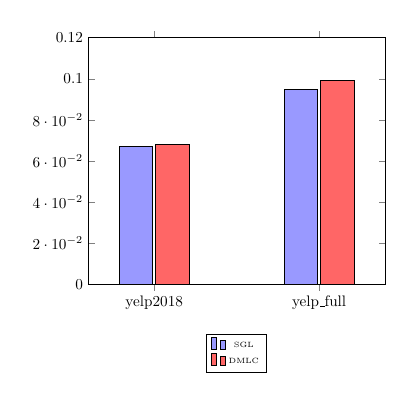
\begin{tikzpicture}[scale=0.55]
        \begin{axis}[ybar,bar width=22pt,
          symbolic x coords={yelp2018, yelp\_full},
          xtick=data,ymin=0,ymax=0.12,
          enlarge x limits=0.4,
          legend style={at={(0.5,-0.2)},anchor=north,font=\tiny}]
          \addplot[fill=blue!40] coordinates {(yelp2018,0.0670)(yelp\_full,0.0947)};
          \addplot[fill=red!60] coordinates {(yelp2018,0.0682)(yelp\_full,0.0992)};
          \legend{SGL, DMLC}
        \end{axis}
      \end{tikzpicture}
    \end{column}
    \begin{column}{0.48\textwidth}
      \textbf{NDCG@20}
      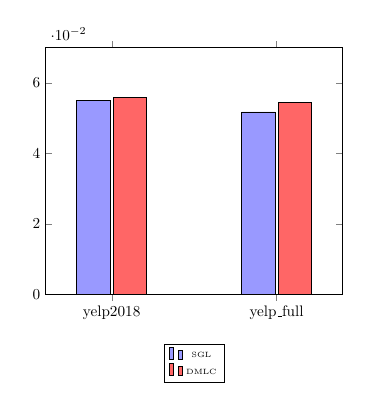
\begin{tikzpicture}[scale=0.55]
        \begin{axis}[ybar,bar width=22pt,
          symbolic x coords={yelp2018, yelp\_full},
          xtick=data,ymin=0,ymax=0.07,
          enlarge x limits=0.4,
          legend style={at={(0.5,-0.2)},anchor=north,font=\tiny}]
          \addplot[fill=blue!40] coordinates {(yelp2018,0.0550)(yelp\_full,0.0518)};
          \addplot[fill=red!60] coordinates {(yelp2018,0.0558)(yelp\_full,0.0545)};
          \legend{SGL, DMLC}
        \end{axis}
      \end{tikzpicture}
    \end{column}
  \end{columns}

  \vspace{0.3em}
  \begin{table}\centering\footnotesize
    \begin{tabular}{lrrrr}
      \toprule
      数据集 & 指标 & SGL (基线) & DMLC (本文) & 提升 \\
      \midrule
      \multirow{2}{*}{yelp2018} & Recall@20 & 0.0670 & \textbf{0.0682} & +1.8\% \\
      & NDCG@20 & 0.0550 & \textbf{0.0558} & +1.5\% \\
      \multirow{2}{*}{yelp\_full} & Recall@20 & 0.0947 & \textbf{0.0992} & +4.8\% \\
      & NDCG@20 & 0.0518 & \textbf{0.0545} & +5.2\% \\
      \bottomrule
    \end{tabular}
  \end{table}
\end{frame}

%% ==================== 总结 ====================
\section{总结}
\begin{frame}{总结}
  \begin{columns}[t]
    \begin{column}{0.55\textwidth}
      \textbf{DMLC 三个创新点:}
      \begin{enumerate}\footnotesize
        \item \textbf{MLC:} 每层 GCN 分别做 InfoNCE
        \item \textbf{SSL Warmup:} 前 10 epoch 权重 0$\to$1 线性增长
        \item \textbf{层加权:} 强调深层语义 $(l\geq2)$
      \end{enumerate}
    \end{column}
    \begin{column}{0.45\textwidth}
      \textbf{最优成绩:}
      \begin{itemize}\footnotesize
        \item yelp2018: \textbf{+1.8\%}
        \item yelp\_full: \textbf{+4.8\%}
      \end{itemize}
    \end{column}
  \end{columns}
\end{frame}

\end{document}
